\chapter{Нейронные сети} \label{chap:tensornet}
Искусственные нейронные сети опережают другие подходы во многих задачах распознавания образов, распознавания речи, перевода, и т.п. [CITE TODO]
Причиной успеха этого класса моделей является их большая гибкость и доступность большого количества вычислительных ресурсов (таких как кластеры графических ускорителей GPU).
И, хотя искусственные нейросети успешно применяются в промышленности (в машинном переводе, прототипах беспилотных автомобилей, умных камерах позволяющих получать снимки более высокого качества благодаря комбинированию нескольких кадров, и т.д.), их использования в мобильных и встроенных устройствах без доступа к интернету остается ограниченным.

Причина этому -- высокие требования к доступной памяти, вычислительной мощности и использованию аккумулятора. Например, популярная на сегодняшний день модель VGG-16 потребляет [TODO].

В связи с этим многие работы были посвящены задачам сжатия и ускорения нейронных сетей. Обратите внимание, что размер требуемой памяти является одним из ограничивающих факторов к снижению энергопотребления моделей. Так, при использовании 45 нм техпроцесса по технологии КМОП, требуется 0.9 пДж чтобы сложить два 32-битных числа с плавающей точкой, доступ к одному 32-битному числу в кэше SRAM требует 5 пДж, и доступ к 32-битному числу в оперативной памяти требует 640 пДж, что на три порядка больше по сравнению с операцией сложения. Большие нейросети не помещаются в кэш процессора и таким образом требует ресурсоемкого доступа к оперативной памяти.

В данной главе представлен тензорный подход к сжатию и ускорению (а значит и снижению энергопотребления) нейронных сетей, а так же модель рекурентной нейронной сети которую можно обучать при помощи римановой оптимизации, что позволяет добиться более высокой скорости обучения по сравнению с аналогами.

\section{Обзор существующих подходов к сжатию нейронных сетей} \label{sec:tensornet-alternatives}
В современных нейронных сетях до 99\% памяти занимают веса полносвязных слоев. В связи с этим, многие работы ставили своей целью исследование возможности сжатия полносвязных слоев. Одним из первых рассмотренных подходов к сжатию стало ограничение ранга матрицы полносвязного слоя~\cite{Denil2013predicting}. Ограничение случайного подмножества элементов матрицы так, чтобы все элементы каждого подмножества имели одно и то же значение~\cite{chen2015compressing} позволило сжимать полносвязные слои в 8 раз без потери качества. Так же рассматривалась более общая постановка, в которой ограничивалось число возможных значений которые могут принимать различные элементы матрицы~\cite{gong2014PQcompressing}. Было показано, что использование 16-битный чисел с плавающей точкой вместо 64-битных  для хранения параметров нейросети возможно без потери качества классификации, что соответсвует сжатию сети в 4 раза~\cite{Gupta2015floatingPoint}.

Метод предложенный в данной диссертации больше всего похож на низгоранговый подход~\cite{Denil2013predicting}, однако вместо ограничения матричного ранга матрицу слоя рассматривается как многомерный линейный оператор и ограничивается ее ТТ-ранг.



\section{Тензорный алгоритм сжатия} \label{sec:tensornet-tt-cnn}
В данном разделе описывается тензорный формат сжатия полносвязных слоев нейросети. Рассмотрим линейную часть функционального преобразования полносвязного слоя:
\begin{equation}
  \label{eq:tensornet-linear-layer}
  \vec{y} = \mat{W} x + \vec{b},
\end{equation}
где $\mat{W}$ -- это матрица весов, а $\vec{b}$ -- вектор сдвига.
Рассмотрим как изменится преобразование~\ref{eq:tensornet-linear-layer} при использовании ТТ-формата для представления матрицы весов~$\mat{W}$. Напомним, что ТТ-формат для матриц задается особым образом, заключающемся в построения вектор-индексов строк и столбцов ($i \leftrightarrow (i_1, \ldots, i_d)$, $j \leftrightarrow (j_1, \ldots, j_d)$) и построении ТТ-формата для тензора $\tens{W}$ получающегося путем перестановки и группировки индексов в исходной матрице (см. раздел~\ref{sec:tt-decomposition}).
Для удобства обозначений, рассмотрим так же тензорную версию вектора сдвига $\vec{b}$: $\tensel{B}_{i_1, \ldots, j_d} = b_j$
\begin{equation}
% \begin{aligned}
\label{eq:tensornet-layer-output-detailed}
\tensel{Y}_{i_1, \ldots, i_d} =
%\sum_{\vec{j}} W (\vec{i}; \vec{j}) x_s(\vec{j}) + b(\vec{i}) = \\
\sum_{j_1, \ldots, j_d}  \!\!\mat{G}_1[i_1, j_1] \dots \mat{G}_d[i_d, j_d]\, \tensel{X}_{j_1,\ldots,j_d} + \tensel{B}_{i_1,\ldots,i_d}.
% \end{aligned}
\end{equation}

Сложность вычисления выхода линейного слоя параметризованного матрицей в ТТ-формате~\eqref{eq:tensornet-layer-output-detailed} составляет $O(d r^2 m \max\{m, n\}^d) = O(d r^2 m \max\{M, N\})$~(см. таблицу~\ref{tbl:complexity-comparison}).


\begin{table}\begin{center}
    \begin{tabular}{ l | l | l }
    %hline
    Операция & Время & Память \rule{0pt}{1.0\normalbaselineskip} \\ \hline
    Полносвязный слой & $O(M N S)$ & $O(M N + N S + M S)$ \rule{0pt}{1.0\normalbaselineskip}\\ %\hline
    ТТ-слой & $O(d r^2 m \max\{M, N\} S)$ & $O(r \max\{M, N\} S)$ \\ %\hline
    \end{tabular}
    \end{center}
    \caption{Сравнение асимптотической сложности и требований по памяти перемножения обычной и ТТ-матрицы размера $M \times N$ на обучную матрицу размера $N \times S$. Тензорный размер входа и выхода матрицы равен $m_1 \times \ldots \times m_d$ и $n_1 \times \ldots \times n_d$ соответсвенно, $m$ обозначает максимальный размер по всем осям $m = \max_{k = 1 \ldots d} m_k$, а $\rank$ обозначает максимальный ТТ-ранг. \label{tbl:complexity-comparison}}
\end{table}


%Сложность $O(d r^2 n \max\{m, n\}^d) = O(d r^2 n \max\{M, N\})$.

\section{Альтернативная модель рекурентных нейронных сетей}
В данном разделе предлагается модель рекурентной нейросети параметризующаяся едниственным тензором в ТТ-формате. Так как множество тензоров фиксированного ТТ-ранга образует гладкое многообразие, такую модель становится возможным обучать с помощью римановой оптимизации, что позволяет ускорить обучение по сравнению с обычными методами оптимизации нейросетей такими как стохастический градиентный спуск.

\subsection{Предлагаемая модель}
Перед тем как ввести предлагамую модель в общем виде, рассмотрим частный случай когда объекты обучающей выборки описываются $3$ признаками. Предлагаемая модель представляет собой полином который включает по одному слагаемому для каждого подмножества признаков и в случае $3$-х мерных объектов выглядит следующим образом
\begin{equation}
\label{eq:polynomial-model-example}
\begin{aligned}
\widehat{y}(\vec{x}) &= \tensel{W}_{000} + \tensel{W}_{100} \,\, x_1 + \tensel{W}_{010} \,\, x_2 + \tensel{W}_{001} x_3 \\
&+ \tensel{W}_{110} \,\, x_1 x_2 + \tensel{W}_{101} \,\, x_1 x_3 + \tensel{W}_{011} \,\, x_2 x_3 \\
&+ \tensel{W}_{111} \,\, x_1 x_2 x_3.
\end{aligned}
\end{equation}
Обратите внимание, что все перестановки признаков в каждом слагаемом (например $x_1 x_2$ и $x_2 x_1$) соответсвуют лишь одному слагаемому с одним настраиваемым весом (например $\tensel{W}_{110}$).

В общем случае, подмножества признаков индексируются $d$-мерным бинарным вектором $(i_1, \ldots, i_d)$, где $i_k = 1$ тогда и только тогда когда $k$-ый признак принадлежит данному подмножеству. Используя данные обозначение, уравнение задающее модель в общем виде записывается следующим образом
\begin{equation}
\label{eq:polynomial-model}
\widehat{y}(\vec{x}) = \sum_{i_1=0}^1 \ldots \sum_{i_d=0}^1 \tensel{W}_{i_1 \ldots i_d} \prod_{k=1}^d x_k^{i_k}.
\end{equation}
В данных обозначениях подразумевается что $0^0 = 1$.
Таким образом, модель параметризуется $d$-мерным тензором~$\tens{W}$ состоящем из $2^d$ элементов.

Обратите внимание, что уравнение модели линейно относительно тензора параметров $\tens{W}$. Чтобы подчеркнуть этот факт уравнение~\eqref{eq:polynomial-model} можно переписать через скалярное произведение тензоров $\widehat{y}(\vec{x}) = \langle \tens{X}, \tens{W} \rangle$, где тензор $\tens{X}$ определяется следующим образом
\begin{equation}
\label{eq:X-definition}
\tensel{X}_{i_1 \ldots i_d} = \prod_{k=1}^d x_k^{i_k}.
\end{equation}
Обратите внимание, что в отличие от линейной модели~\eqref{eq:linear-model} в уравнение~\eqref{eq:polynomial-model} не требуется отдельный параметр сдвига $b$, так как сдвиг уже включен в модель в виде параметра~$\tensel{W}_{0 \ldots 0}$ (см. пример уравнения модели~\eqref{eq:polynomial-model-example}).
Основная идея предлагаемой модели состоит в компактном представлении экспоненциально большого тензора параметров~$\tens{W}$ в ТТ-формате.

\subsection{Быстрый метод вывода \label{sec:exm-inference}}
В данном разделе показывается как вычислять уравнение модели~\eqref{eq:polynomial-model} за линейное число вычислительных операций от числа признаков $d$. Линейная сложность достигается благодаря ТТ-представлению тензора параметров~$\tens{W}$ и тензора объекта~$\tens{X}$~\eqref{eq:X-definition} в ТТ-формате с низкими рангами. 
Во время обучения тензор параметров~$\tens{W}$ инициализируются и обучается в ТТ-формате и его ТТ-ранг можно контролировать напрямую. В самом деле, следующие ТТ-ядра дают точное представление тензора~$\tens{X}$
\begin{equation*}
G_k[i_k] = x_k^{i_k} \in \mathbb{R}^{1 \times 1}, ~~ k=1, \ldots, d.
\end{equation*}
Так как $k$-ое ядро $G_k[i_k]$ представимо в виде матрицы размера $1 \times 1$ для любого значения индекса $i_k \in \{0, 1\}$, следовательно ТТ-ранг тензора~$\tens{X}$ равняется~$1$.

Как было показано в работе~\cite{oseledets2011ttMain}, скалярное произведение между двумя ТТ-тензорами с рангами $\rank$ и $1$ и размером каждой оси $2$ можно вычислить за время пропорциональное~$O(\rank^2 d)$. Покажем применение этого общего принципа для модели~\eqref{eq:polynomial-model}, так как в данном частном случае оно приводит к простым и элегентным формулам.

Перепишем уравнение модели~\eqref{eq:polynomial-model} предполагая что тензор $\tens{W}$ представлен в ТТ-формате.
\begin{equation*}
\begin{aligned}
\widehat{y}(\vec{x}) &= \sum_{i_1, \ldots, i_d} \tensel{W}_{i_1 \ldots i_d} \, \left ( \prod_{k=1}^d x_k^{i_k} \right )\\
&= \sum_{i_1, \ldots, i_d} G_1[i_1] \ldots G_d[i_d] \left ( \prod_{k=1}^d x_k^{i_k} \right ).
\end{aligned}
\end{equation*}

Сгруппируем множители зависящие от переменной $i_k$, $k=1, \ldots, d$
\begin{equation*}
%\label{eq:fast-model-equation}
\begin{aligned}
\widehat{y}(\vec{x}) &= \sum_{i_1, \ldots, i_d}  x_1^{i_1} G_1[i_1] \ldots x_d^{i_d} G_d[i_d]\\
&= \left ( \sum_{i_1=0}^1 x_1^{i_1} G_1[i_1] \right ) \ldots \left ( \sum_{i_d=0}^1 x_d^{i_d} G_d[i_d] \right )\\
&= \underbrace{A_1}_{1 \times \rank} \underbrace{A_2}_{\rank \times \rank} \ldots \underbrace{A_d}_{\rank \times 1},
\end{aligned}
\end{equation*}
где матрицы $A_k$ для $k=1, \ldots, d$ определены следующим образом
\begin{equation*}
A_k = \sum_{i_k=0}^1 x_k^{i_k} G_k[i_k] = G_k[0] + x_k G_k[1].
\end{equation*}
Итоговое значение $\widehat{y}(\vec{x})$ может быть вычислено с помощью $d-1$ матрично-векторных произведений и одного скалярного произведения векторов, что приводит к асимптотической сложности $O(r^2 d)$.

\subsection{Методы обучения}
Обучение модели~\eqref{eq:polynomial-model} соответсвует минимизации следующей (регуляризованной) функции потерь с ограничение на ТТ-ранг тензора параметров
\begin{equation}
\label{eq:TT-loss-minimization}
\begin{aligned}
& \underset{\tens{W}}{\text{minimize}}
& & L(\tens{W}), \\
& \text{subject to}
& & \ttrank(\tens{W}) = r_0,
\end{aligned}
\end{equation}
где функция потерь задана следующим образом
\begin{equation}
\label{eq:TT-loss}
L(\tens{W}) = \sum_{f=1}^N \ell\left(\langle \tens{X}^{(f)}, \tens{W} \rangle,\, y^{(f)}\right) + \frac{\lambda}{2} \norm{\tens{W}}^2_F.
\end{equation}

Рассмотрим два подхода к решению оптимизационной задачи~\eqref{eq:TT-loss-minimization}.
В качестве базового подхода, будем минимизировать функцию $L(\tens{W})$ стохастическим градиентным спуском примененнным к параметрам задающим ТТ-представление тензора $\tens{W}$ (элементам ТТ-ядер).

В качестве альтернативного подхода можно было бы рассмотреть (стохастический) градиентный спуск примененный к самому тензору~$\tens{W}$. В рамках такого подхода на каждой итерации следовало бы вычитать градиент функции потерь из текущего значения тензора~$\tens{W}$. ТТ-формат действительно позволяет вычитать тензоры, но это приводит к росту ТТ-рангов на каждой итерации, а операция ТТ-округления для контроля роста рангов имеет сложность кубическую по рангу. Как будет показано далее, ТТ-ранг градиента функции потерь пропорционален числу объектов обучающей выборки рассматриваемых на данной итерации, и может достигать сотен, что делает такой подход непрактичным.

Для получения более эффективного метода оптимизации далее в этом разделе будет рассмотрен метод римановой оптимизации.
Экспериментально преимущество римановой оптимизации над стохастическим градиентным спуском для данной задачи показано в разделе~\ref{sec:exp-riemannian-optimization}.

\subsubsection{Справка по методам римановой оптимизации \label{sec:riemannian-help}}
Данный раздел является обзорным, и в нем приведена основная информация по методам римановой оптимизации используемая далее.

Ключевым понятием в римановой оптимизации является \emph{гладкое многообразие}. Пусть $\mathcal{U} \subset \mathbb{R}^n$ и $\mathcal{V} \subset \mathbb{R}^m$ это открытые множества. Отображение $f: \mathcal{U} \to \mathcal{V}$ называется гладким если $f$ бесконечно непрерывно диффиренцируемый. Биективное отображение $f$ называют \emph{диффеоморфизмом} если и $f$ и обратное отображение $f^{-1}$ являются гладкими. Множества $\mathcal{U}$ и $\mathcal{V}$ в таком случае называют \emph{диффеоморфными}.

Пусть $\mathcal{M} \subset \mathbb{R}^n$ это некоторая поверхность в $\mathbb{R}^n$. Основная идея введения понятия гладкого многообразия состоит в том, чтобы построить соответствие между участками поверхности $\mathcal{M}$ и евклидовом множеством $\mathbb{R}^m$ чтобы свести операции над $\mathcal{M}$ к операциям над $\mathbb{R}^m$. Данная идея иллюстрируется на Рис.~\ref{fig:manifold-def}, а формальное определение дается ниже:
\begin{definition}
	\cite{RS13, Def. 1.3} Множество $\mathcal{M} \subset \mathbb{R}^n$ называют гладким подмногообразием $\mathbb{R}^n$ если для любого $x \in \mathcal{M}$	 найдется открытая окрестность $\mathcal{U} \subset \mathbb{R}^n$ такая, что $\mathcal{U} \cap \mathcal{M}$ диффеоморфно открытому подмножеству $\mathcal{V} \subset \mathbb{R}^m$. Диффеоморфизм $\phi: \mathcal{U} \cap \mathcal{M} \to \mathcal{V}$ называют атласом многообразия $\mathcal{M}$.
\end{definition}

\begin{figure}[t]
% \vskip 0.2in
\begin{center}
  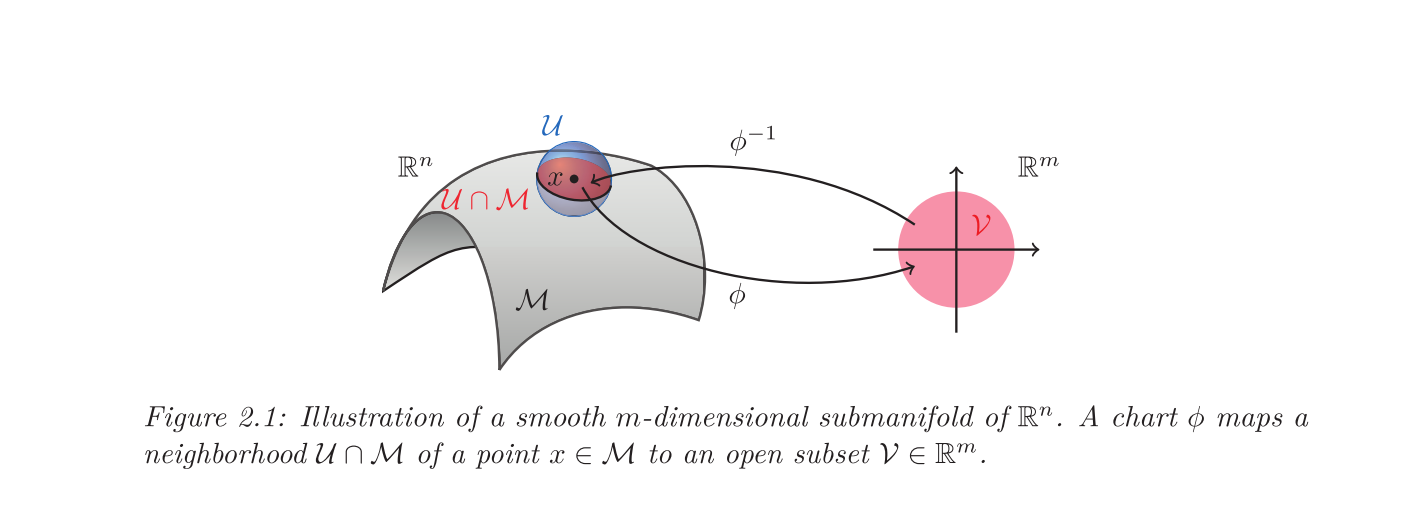
\includegraphics[width=0.8\textwidth]{images/manifold_def.png}
  \caption{\alert{TODO: перерисовать} Иллюстрация гладкого $m$-мерного многообразия в $\mathbb{R}^n$. Атлас $\phi$ отображает окрестность  $\mathcal{U} \cap \mathcal{M}$ точки $x \in \mathcal{M}$ в открытое подмножество $\mathbb{R}^n$. \label{fig:manifold-def}}
  \end{center}
  % \vskip -0.2in
\end{figure}

В работе~\cite{holtz2012manifolds} было показано, что множество $d$-мерных тензоров фиксированного размера и с фиксированными ТТ-рангами $\rank$
\begin{equation*}
% \label{eq:TT-manifold}
\mathcal{M}_r = \{\tens{W} \in \mathbb{R}^{n_1 \times  \ldots \times n_d}\!:\, \ttrank(\tens{W})=\rank\}
\end{equation*}
образует гладкое многообразие.

В каждой точке $x \in \mathcal{M}$ гладкого многообразия $\mathcal{M}$ можно построить \emph{касательное пространство}, интуитивно которое можно представлять как плоскость ортогональную поверхности $\mathcal{M}$ в данной точке (см. Рис.~\ref{fig:tangent-space}). Формально, касательное пространство определяется следующим образом
\begin{definition}
	\cite{RS13, Def. 1.21} Пусть $\mathcal{M} \subset \mathbb{R}^n$ это гладкое $m$-мерное подмногообразие. Вектор $\xi \in \mathbb{R}^n$ называют касательным вектором многообразия $\mathcal{M}$ в точке $x \in \mathcal{M}$ если найдется гладкая кривая $\gamma: \mathbb{R} \to \mathcal{M}$ такая что
\[
\gamma(0) = x, ~~ \gamma'(0) = \lim_{t \to 0} \frac{\gamma(t) - \gamma(0)}{t} = \xi.
\]
Множество касательных векторов $\mathcal{M}$ в точке $x$,
\[
T_x \mathcal{M} := \{\gamma'(0) \mid \gamma : \mathbb{R} \to \mathcal{M} \text{ является гладким}, \gamma(0) = x\},
\]
называется касательным пространством $\mathcal{M}$ в точке $x$.
\end{definition}

\begin{figure}[t]
\begin{center}
  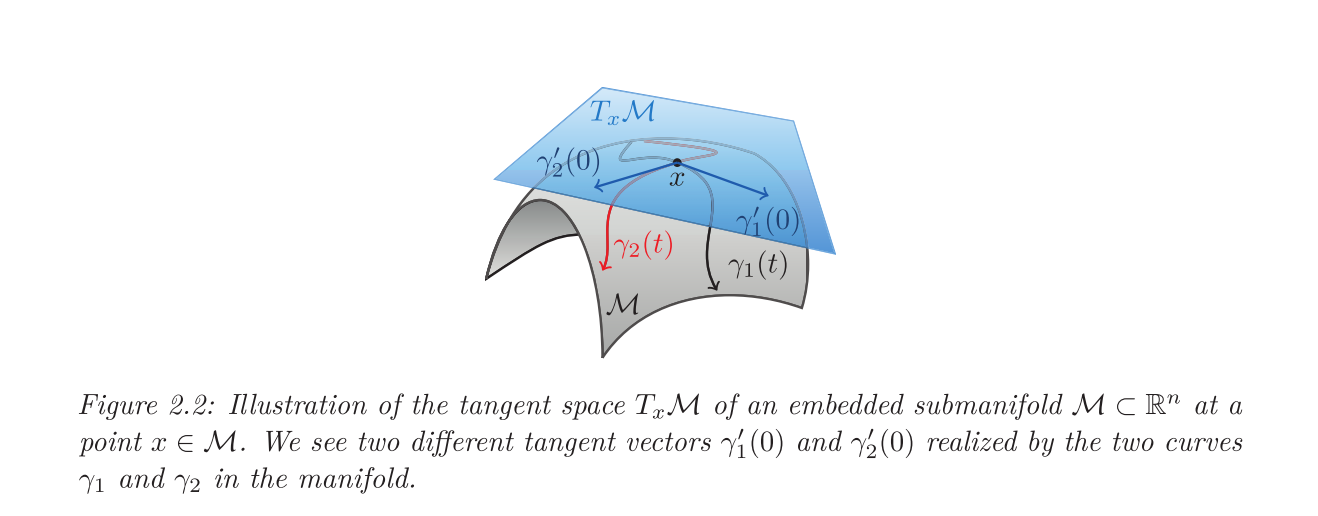
\includegraphics[width=0.8\textwidth]{images/tangent_space.png}
  \caption{\alert{TODO: перерисовать} Иллюстрация касательного пространства $T_x \mathcal{M}$ подмногообразия $\mathcal{M} \subset \mathbb{R}^n$ в точке $x \in \mathcal{M}$. Два различных вектора $\gamma_1'(0)$ и $\gamma_2'(0)$ реализуются двумя различными кривыми $\gamma_1$ и $\gamma_2$ на многообразие. \label{fig:tangent-space}}
  \end{center}
\end{figure}

\begin{definition}
	\cite \emph{Касательным расслоением} гладкого многообразия $\mathcal{M}$ называется множетство пар
	\[
	T\mathcal{M} = \{(x, \xi) \mid x \in \mathcal{M}, \xi \in T_x \mathcal{M}\}
	\]
\end{definition}

Как показано в работе~\cite{Steinlechner2016}, касательное пространство $T_{\tens{W}} \mathcal{M}_{\rank}$ многообразия тензоров фиксированного ТТ ранга $\mathcal{M}_r$ в точке $\tens{W} \in \mathcal{M}_r$ можно определить как множество тензоров $\tens{Y}$ ТТ-ранга не превосходящего $2 \rank$ определяемых следующими ТТ-ядрами для $k = 2, \ldots, d-1$
\begin{equation}
	\label{eq:tangent-space}
	G_1^{\tens{Y}}[i_1] = \begin{bmatrix}
	\delta \widetilde{U}_1[i_1] & U_1[i_1]
	\end{bmatrix}, ~~ G_k^{\tens{Y}}[i_k] = \begin{bmatrix}
	V_k[i_k] & 0\\
	\delta \widetilde{U}_k[i_k] & U_k[i_k]\\
	\end{bmatrix}, ~~ G_d^{\tens{Y}}[i_d] = \begin{bmatrix}
	V_d[i_d]\\
	\delta \widetilde{U}_d[i_d]\\
	\end{bmatrix},
\end{equation}
где матрицы $U_k[i_k]$ и $V_k[i_k]$, $k = 1, \ldots, d$ это результат ортогонализации ядра $G^{\tens{W}}_k[i_k]$ слева-на-право и справо-на-лево соответственно (детали по поводу правой и левой ортогонализации см. в работе~\cite{oseledets2011ttMain}), а матрицы $\delta \widetilde{U}_k[i_k]$ это произвольные матрицы размера $\rank_{k-1} \times \rank_k$.

Обратите внимание, что положив $\delta \widetilde{\tens{U}}_d = \tens{V}_d$, и  $\delta \widetilde{U}_k[i_k] = \mat{0}$ для всех $k = 1, \ldots, d-1$, выражение для элемента касательной плоскости $\tens{Y}$ совпадает с $\tens{W}$. Таким образом, элемент тензор в ТТ-формате всегда принадлежит своему касательному пространству $\tens{W} \in T_{\tens{W}} \mathcal{M}_{\rank}$.

Резльтатом действия на тензор $\tens{Z}$ оператора ортопроекции на касательную плоскость $T_x \mathcal{M}_{\rank}$ многообразия $\mathcal{M}_{\rank}$ в точке $\tens{W}$ является тензор $\tens{Y} = P_{T_{\tens{W}} \mathcal{M}_{\rank}} \tens{Z}$ чье ТТ-представление можно записать в виде~\eqref{eq:tangent-space} где матрицы $\delta \widetilde{U}_k[i_k]$ определяются следующим образом~\cite{lubich2015time}
\[
\delta \widetilde{\mat{U}}_k^L = (I_{\rank_{k-1}n_k} - \mat{U}^L_k (\mat{U}^L_k)^\intercal) (I_{n_k} \otimes \mat{W}_{\leq k-1})^\intercal \mat{Z}^{\langle k \rangle} \mat{W}_{\geq k+1}
\]
где $\delta \widetilde{\mat{U}}_k^L$ это матрица получаемая из ядра $\delta \widetilde{\tens{U}}_k$ путем объединения первых двух индексов: $(\delta \widetilde{U}_k^L)_{\alpha_{k-1} i_k, \alpha_k} = (\delta \widetilde{\tensel{U}}_k)_{\alpha_{k-1}, i_k, \alpha_k}$; $I_{\rank_{k-1}n_k}$ -- единичная матрицы размера $\rank_{k-1}n_k \times \rank_{k-1}n_k$; $\mat{W}_{\leq k-1}$ матрица, получающаяся в результате перемножения первых $k-1$ TT-ядер тензора $\tens{W}$ ортогонализованных слева-направо: $(W_{\leq k-1})_{i_1 \ldots i_{k-1}, \alpha_{k-1}} = \sum_{\alpha_0, \ldots, \alpha_{k-2}} U_1[i_1](\alpha_0, \alpha_1) \ldots U_{k-1}[i_{k-1}](\alpha_{k-2}, \alpha_{k-1})$; а  $\mat{Z}^{\langle k \rangle}$ -- матрица размера $\prod_{k=1}^k n_k \times \prod_{i=k+1}^d n_k$ получающаяся в результате объединения первых k и последних $d-k$ индексов тензора $Z^{\langle k \rangle}_{i_1 \ldots i_k, i_{k+1} \ldots i_d} = Z_{i_1, \ldots, i_k, i_{k+1}, \ldots, i_d}$.

Можно показать~\cite{RS13, Thm. 1.23}, что касательное пространство гладкого многообразия $T_x \mathcal{M}$ образует линейное подпространство размерности $m$ в $\mathbb{R}^n$. Снабдив данное векторное пространство скалярным произведение $g_x : T_x \mathcal{M} \times T_x \mathcal{M} \to \mathbb{R}$ можно измерять расстояния и углы.

Гладкое отображение $\xi : \mathcal{M} \to \mathbb{R}^n$ которое ставит в соответствие элемент касательного пространства $\xi(x) \in T_x \mathcal{M}$ любой точке $x \in \mathcal{M}$ называется \emph{векторным полем}. Если отображение
\[
\mathcal{M} \to \mathbb{R}, ~~~ x \mapsto g_x(\xi(x), \eta(x)),
\]
является гладким для любой пары векторных полей $\xi, \eta$ в $\mathcal{M}$, тогда $g_x$ называется \emph{римановой метрикой} (обратите внимание, что $g_x$ при этом является скалярным произведением, а не метрикой). Гладкое многообразие $\mathcal{M}$ снабженное римановой метрикой $g_x$ называется \emph{римановым многообразием}.

Гладкое многообразие тензоров фиксированного ТТ-ранга $\mathcal{M}_r$ можно снабдить римановой метрикой $g_x(\tens{A}, \tens{B}) = \langle \tens{A}, \tens{B} \rangle$, которая не зависит от точки $x$ и совпадает с обычным скалярным произведение тензоров $\tens{A}$ и $\tens{B}$.

Для построения итерационных процессов на римановых многообразиях так же требуется понятия \emph{ретракции}. Пусть на текущей итерации $t$ некоторого метода оптимизации требуется совершить шаг от текущей точки $\tens{W}_t$ в сторону вектора $\tens{G} \in T_{\tens{W}_t} \mathcal{M}$ из касательного пространства. Результат этой операции $\tens{W}_t + \alpha \tens{G}$ вообще говоря больше не принадлежит многообразию $\mathcal{M}$. Поэтому в в теории римановой оптимизации вводят понятие \emph{экспоненциальных отображений}, которые по точке $\tens{W}_t$ и направлению $\tens{G}$ могут вычислить точку $\tens{W}_{t+1} \in \mathcal{M}$ такую, кратчайшая геодезическая между точками $\tens{W}_t$ и $\tens{W}_{t+1}$ совпадает по направлению и длине с вектором $\tens{G}$. Однако на практике вычисления экспоненциального отображения часто сопряжено с большими вычислительными затратами, в связи с чем вводят понятие \emph{ретракции}, которое можно интерпритировать как вычислительно более эффективную аппроксимацию экспоненциального отображения
\begin{definition}
	\cite{AM12, Def. 1} Пусть $\mathcal{M}$ образует гладкое подмногообразие $\mathbb{R}^n$. Отображение элементами касательного расслоения и элементами многообразия $R : T\mathcal{M} \to \mathcal{M}$ называют \emph{ретракцией} в точке $x \in \mathcal{M}$ если существует окрестность $\mathcal{U}$ точки $(x, 0) \in T \mathcal{M}$ такая, что выполнены следующие свойства
	\begin{enumerate}
		\item $\mathcal{U} \subset \text{dom}(R)$ и отображение $R : \mathcal{U} \to \mathcal{M}$ является гладким;
		\item $R(x, 0) = x$ для всех $x \in \mathcal{U}$;
		\item $\lim_{t \to 0} \frac{R(x, t \xi) - x}{t} = \xi$ для всех $x \in \mathcal{M}$ и $\xi \in T_x \mathcal{M}$.
	\end{enumerate}
\end{definition}

\begin{figure}[t]
\begin{center}
  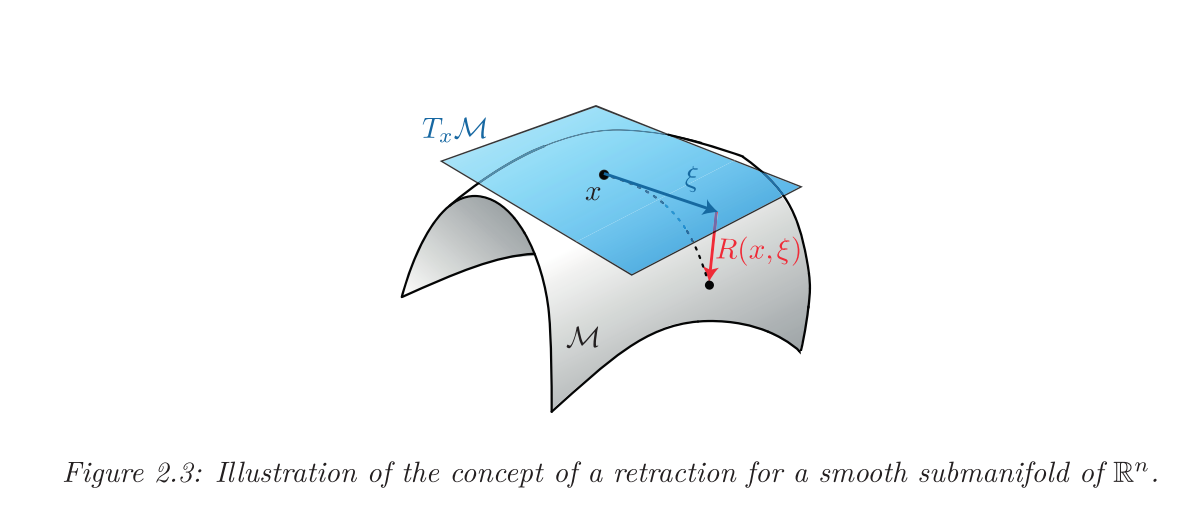
\includegraphics[width=0.8\textwidth]{images/retraction.png}
  \caption{\alert{TODO: перерисовать} Иллюстрация идеи ректракции на гладком подмногообразие $\mathbb{R}^n$. \label{fig:retraction}}
  \end{center}
\end{figure}

В дальнейшем, в качестве ретракции на многооборазие тензоров фиксированного ТТ-ранга $\mathcal{M}_{\rank}$ будет рассматриваться операция округления $R(x, \xi) = \ttround(x + \xi, \rank)$.


\subsubsection{Риманова оптимизация для задачи~\eqref{eq:TT-loss-minimization} \label{sec:exm-riemannian-optimization}}

Как было отмечено выше, множество тензоров фиксированного ТТ-ранга образует риманово многообразие, что делает возможным применение аппарата римановой оптимизации для решения задачи~\eqref{eq:TT-loss-minimization}.
Метод риманового градиентного спуска состоит из следующих шагов повторяемых до сходимости (см. Рис.~\ref{fig:riemannian-illustration}):
\begin{enumerate}
\item (Проекция градиента.) Спроектировать градиент $\frac{\partial L}{\partial \tens{W}_t}$ на касательное пространство $\mathcal{M}_r$ текущей точки $\tens{W}_t$: $\tens{G}_t = P_{T_{\tens{W}_t} \mathcal{M}_r}(\frac{\partial L}{\partial \tens{W}_t})$.
\item (Ретракция.) Сделать шаг вдоль проекции градиента $\tens{G}$ с некоторой длиной шага~$\alpha_t$ (данная операция увеличивает ТТ-ранг) и округлить результат обратно до ранга $\rank$: $\tens{W}_{t+1} = \ttround(\tens{W}_t - \alpha_t \tens{G}_t, \rank)$.
\end{enumerate}
Далее описано как реализовать каждый из перечисленных выше шагов.

\begin{figure}[t]
% \vskip 0.2in
\begin{center}
  \resizebox{0.5\textwidth}{!}{
  \def\svgwidth{7cm}
  \normalsize
  \includesvg{images/manifold}
  }
  \caption{Иллюстрация одного шага риманового градиентного спуска. Шаг $\alpha$ положен в $1$ для наглядности иллюстрации. \label{fig:riemannian-illustration}}
  \end{center}
  % \vskip -0.2in
\end{figure}

Рассмотрим операцию проекции тензора~$\tens{Z}$ на касательное пространство многообразия~$\mathcal{M}_r$ в точке~$\tens{W}$. Он состоит из двух шагов: предобработки тензора~$\tens{W}$, которая может быть выполнена за $O(d \rank^3)$ арифметических операций; и проектирования тензора $\tens{Z}$, которая может быть выполнена за $O(d \rank^2 \ttrank(\tens{Z})^2)$ арифметических операций (\alert{todo: \ref{}}).
При этом, ТТ-ранг проекции ограничен константой не зависящей от ТТ-ранга проектируемого тензора~$\tens{Z}$:
\begin{equation*}
   \ttrank(P_{T_{\tens{W}} \mathcal{M}_r}(\tens{Z})) \leq 2 \ttrank(\tens{W}) = 2 \rank.
\end{equation*}

Рассмотрим градиент функции потерь~\eqref{eq:TT-loss}
\begin{equation}
\label{eq:TT-gradient}
\frac{\partial L}{\partial \tens{W}} = \sum_{f=1}^N \frac{\partial \ell}{\partial \widehat{y}} \tens{X}^{(f)} + \lambda \tens{W}.
\end{equation}

Пользуясь тем фактом, что любой ТТ-тензор принадлежит собственному касательному пространству $P_{T_{\tens{W}} \mathcal{M}_r}(\tens{W}) = \tens{W}$ и тем, что проекция это линейная операция, получаем
\begin{equation}
% \begin{aligned}
\label{eq:riemannian-gradient}
P_{T_{\tens{W}} \mathcal{M}_r}\left ( \frac{\partial L}{\partial \tens{W}} \right) = \sum_{f=1}^N \frac{\partial \ell}{\partial \widehat{y}} P_{T_{\tens{W}} \mathcal{M}_r}(\tens{X}^{(f)}) + \lambda \tens{W}.
% \end{aligned}
\end{equation}
Таким образом, проекция градиента является взвешенной суммой проекций тензоров $\tens{X}^{(f)}$, при этом все эти проекции могут быть выполнены параллельно.
Отметим так же, что ТТ-ранг данных тензоров равен~$1$ (см. раздел~\ref{sec:exm-inference}), поэтому вычислительная сложность подсчета $N$ проекций составляет $O(d \rank^2 (\rank + N))$.
При этом ТТ-ранг проекции градиента  не превышает $2 \rank$ не зависимо от размера обучающей выборки~$N$.

Отметим так же, что для построения алгоритма вычисления проекции градиента использовался конкретный выбор члена отвещающего за регуляризацию. При выборе члена регуляризации отличного от  $L_2$ (например $L_1$), сложность вычисления проекции градиента может возрасти.

Чтобы метод стал применим к выборкам состоящим из большого числа объектов, будет применяться стохастическая версия риманового градиентного спуска: на каждой итерации выбирается случайное подмножество объектов обучающей выборки, вычисляется проекция градиента слагаемых функции потерь отвечающих выбранным объектам, делается шаг по направлению проекции градиента и результат снова округляется до ранга $\rank$ (см. алгоритм~\ref{alg:rimeannian-optimization}).

Вычислительная сложность одной итерации стохастического риманового градиентного спуска для задачи~\eqref{eq:TT-loss-minimization}) сотавляет $O(dr^2(r + M))$ арифметических операций и состоит из $O(dr^2M)$ операций для подсчет скалярных произведений,  $O(dr^2(r + M))$ операций для вычисления проекции градиента и $O(dr^3)$ для ТТ-округлений, где $M$ это число объектов использующихся на каждой итерации метода.


\begin{algorithm}[t]
   \caption{Риманов градиентный спуск для задачи~\eqref{eq:TT-loss-minimization}}
   \label{alg:rimeannian-optimization}
\begin{algorithmic}
   \REQUIRE Обучающая выборка $\{(\vec{x}^{(f)}, y^{(f)})\}_{f=1}^N$, требуемый ТТ-ранг $\rank_0$, число итераций~$T$, размер мини-батча~$M$, шаг обучения~$\alpha$, сила регуляризатора~$\lambda$
   \ENSURE $\tens{W}$ приближенно решающий задачу~\eqref{eq:TT-loss-minimization}
   \STATE Обучить линейную модель~\eqref{eq:linear-loss} и получить параметры $\vec{w}$ и $b$
   \STATE Инициализировать тензор $\tens{W}_0$ с ТТ-рангом равным $\rank_0$ используя $\vec{w}$ и $b$  (см. раздел~\ref{sec:exm-initialization})
   \FOR{$t := 1$ {\bfseries to} $T$}
        \STATE Случайно выбрать $M$ индексов $h_1, \ldots, h_M \sim \mathcal{U}(\{1, \ldots, N\})$
   	    \FOR{$j := 1$ {\bfseries to} $M$}
	        \STATE Вычислить проекцию $\tens{Q}_j = P_{T_{\tens{W}_{t-1}} \mathcal{M}_r} (\tens{X}^{(h_j)})$
        \ENDFOR
        \STATE $\tens{G}_t := \sum_{j=1}^M \frac{\partial \ell}{\partial \widehat{y}} \tens{Q}_j  + \lambda \tens{W}_{t-1}$
        \STATE $\tens{W}_{t} := \ttround(\tens{W}_{t-1} - \alpha \tens{G}_t, \,r_0)$
   \ENDFOR
\end{algorithmic}
\end{algorithm}


\subsubsection{Инициализация \label{sec:exm-initialization}}
Чтобы избежать преобладания членов высокого порядка во время инициализации модели, обучение модели предлагается инициализировать из так, чтобы модель~\eqref{eq:polynomial-model} совпадала с оптимальной линейной моделью (члены более высоких порядков были равны нулю). Для этого настраиваются веса $\vec{w}, b$ линейной модели с помощью решения (регялризованной) задачи~\eqref{eq:linear-loss}, а веса используются для инициализации весов $\tens{W}$ эквивалентной модели~\eqref{eq:polynomial-model}, причем ТТ-ранг полученного $\tens{W}$ будет равен 2
\begin{theorem}
\label{thm:initialization-rank}
Для любого вектора $\vec{w}$ длины $d$ и параметра сдвига $b$ существует тензор $\tens{W}$ ТТ-ранга $2$ такой, что для любого вектора $\vec{x}$ и соответствующего тензора $\tens{X}$~\eqref{eq:X-definition} скалярные произведения $\langle \vec{x}, \vec{w} \rangle$ и $\langle \tens{X}, \tens{W} \rangle$ равны друг другу. ТТ-ядра тензора~$\tens{W}$ при этом можно построить следующим образом
\begin{equation}
\begin{aligned}
\label{eq:initialization-cores}
G_1[0] &=
\left[
\begin{array}{cc}
1 & 0\\
\end{array}
\right], ~~&
G_1[1] &=
\left[
\begin{array}{cc}
0 & w_1\\
\end{array}
\right], \\
G_d[0] &=
\left[
\begin{array}{c}
b\\
1\\
\end{array}
\right], ~~&
G_d[1] &=
\left[
\begin{array}{c}
w_d\\
0\\
\end{array}
\right], ~~\\[0.2cm]
\forall ~ 2 \leq & ~k \leq d-1 & &\\[-0.05cm]
G_k[0] &=
\left[
\begin{array}{cc}
1 & 0 \\
0 & 1 \\
\end{array}
\right], ~~&
G_k[1] &=
\left[
\begin{array}{cc}
0 & w_k \\
0 & 0 \\
\end{array}
\right],
\end{aligned}
\end{equation} 

\end{theorem}

Начнем с формулировки следующей леммы
\begin{lemma}
  \label{lemma:initialization-rank}
  Для ТТ-ядер~\eqref{eq:initialization-cores} и любого $p = 1, \ldots, d-1$ верно следующее равенство:
  \begin{equation*}
  G_1[i_1] \ldots G_p[i_p] =
  \begin{cases*}
      \begin{array}{ll}
      \left[
      \begin{array}{cc}
      1 & 0\\
      \end{array}
      \right], & \text{if } \sum_{q=1}^p i_q = 0,\\[0.1cm]
      \left[
      \begin{array}{cc}
      0 & 0\\
      \end{array}
      \right], & \text{if } \sum_{q=1}^p i_q \geq 2,\\[0.1cm]
      \left[
      \begin{array}{cc}
      0 & w_k\\
      \end{array}
      \right], & \text{if } \sum_{q=1}^p i_q = 1,\\
                          &~~~~~~\!\text{and}~i_k = 1.
  \end{array}
  \end{cases*}
  \end{equation*}
\end{lemma}

\begin{proof}
  Докажем лемму~\ref{lemma:initialization-rank} индукции. Действительно, для $p = 1$ утверждение леммы становится
  \begin{equation*}
    G_1[i_1] =
    \begin{cases*}
        \begin{array}{ll}
        \left[
        \begin{array}{cc}
        1 & 0\\
        \end{array}
        \right], & \text{if } i_1 = 0,\\[0.1cm]
        \left[
        \begin{array}{cc}
        0 & w_1\\
        \end{array}
        \right], & \text{if } i_1 = 1,
    \end{array}
    \end{cases*}
  \end{equation*}
  верное по определению первого ТТ-ядра $G_1[i_1]$.

  Предположим, что утверждение леммы~\ref{lemma:initialization-rank} верно для некоторого $p - 1 \geq 1$.
  Если $i_p = 0$, тогда $G_p[i_p]$ является еденичной матрицей и $G_1[i_1] \ldots G_p[i_p] = G_1[i_1] \ldots G_{p-1}[i_{p-1}]$. Также, $\sum_{q=1}^p i_q = \sum_{q=1}^{p-1}  i_q$, поэтому равенство сохраняется.

  Если $i_p = 1$, существует $3$ варианта:
  \begin{itemize}
    \item Если $\sum_{q=1}^{p-1} i_q = 0$, тогда $\sum_{q=1}^{p} i_q = 1$ и
    \begin{equation*}
      G_1[i_1] \ldots G_p[i_p] \,=\, \left[
      \begin{array}{cc}
      1 & 0\\
      \end{array}
      \right]
      G_p[1] \,=\, \left[
      \begin{array}{cc}
      0 & w_p\\
      \end{array}
      \right].
    \end{equation*}
    \item Если $\sum_{q=1}^{p-1} i_q \geq 2$, тогда $\sum_{q=1}^{p} i_q\geq 2$ и
    \begin{equation*}
      G_1[i_1] \ldots G_p[i_p] \,=\, \left[
      \begin{array}{cc}
      0 & 0\\
      \end{array}
      \right] G_p[1] \,=\,
      \left[
      \begin{array}{cc}
      0 & 0\\
      \end{array}
      \right].
    \end{equation*}
    \item Если $\sum_{q=1}^{p-1}i_q = 1$ при $i_k = 1$, тогда $\sum_{q=1}^{p}i_q \geq 2$ и
    \begin{equation*}
      G_1[i_1] \ldots G_p[i_p] \,=\, \left[
      \begin{array}{cc}
      0 & w_k\\
      \end{array}
      \right]
      G_p[1] \, =\, \left[
      \begin{array}{cc}
      0 & 0\\
      \end{array}
      \right].
    \end{equation*}
  \end{itemize}
  Что в точности является утверждением леммы~\ref{lemma:initialization-rank}.
\end{proof}


\begin{proof}[Доказательство теоремы \ref{thm:initialization-rank}]
Произведение всех ТТ-ядер может быть представлено как произведение первых $p = d-1$ умноженное на последнее ТТ-ядро $G_d[i_d]$. Используя результат леммы~\ref{lemma:initialization-rank} получаем
\begin{equation*}
\begin{aligned}
\tensel{W}_{i_1 \ldots i_d} ~&=~ G_1[i_1] \ldots G_{d-1}[i_{d-1}] G_{d}[i_{d}]
	\\[0.2cm]
	&=\begin{cases*}
	    \begin{array}{ll}
	    b, & \text{if } \sum_{q=1}^d i_q = 0,\\[0.1cm]
	    0, & \text{if } \sum_{q=1}^d i_q \geq 2,\\[0.1cm]
	    w_k, & \text{if } \sum_{q=1}^d i_q = 1,\\
	                        &~~~~~\,\text{and}~i_k = 1.
	\end{array}
	\end{cases*}
\end{aligned}
\end{equation*}
Элементы тензора $\tens{W}$ которые соответствуют слагаемым степени $\geq 2$ равны нулю; элементы которые соответствуют коээфициенту перед $x_k$ равны $w_k$; элемент соответсвующий сдвигу равен $\tensel{W}_{0 \ldots 0} = b$.

ТТ-ранг полученного тензора не превосходит $2$ так как размеры полученных ТТ-ядер равны $2 \times 2$.
\end{proof}

Экспериментальное сравнение методов инициализации для предложенного метода оптимизации приведено в разделе~\ref{sec:exp-initialization}.

\subsection{Обобщение модели \label{sec:exm-model-extension}}
In this section, we extend the proposed model to handle polynomials of any functions of the features.
As an example, consider the logarithms of the features in the $2$-dimensional case:
\begin{equation*}
  \begin{aligned}
    \widehat{y}^{\,\log}(\vec{x}) =& \,\tensel{W}_{00} + \tensel{W}_{01} x_1 +\tensel{W}_{10} x_2 + \tensel{W}_{11} x_1 x_2\\
    &+\tensel{W}_{20} \,\, \log(x_1) + \tensel{W}_{02} \,\, \log(x_2)\\
    &+ \tensel{W}_{12} \,\, x_1 \log(x_2)+ \tensel{W}_{21} \,\, x_2 \log(x_1)\\
    &+ \tensel{W}_{22} \,\, \log(x_1) \log(x_2).
  \end{aligned}
\end{equation*}
In the general case, to model interactions between $n_g$ functions $g_1, \ldots, g_{n_g}$ of the features we redefine the object-tensor as follows:
\begin{equation*}
\tensel{X}_{i_1 \ldots i_d} = \prod_{k=1}^d c(x_k, i_k),
\end{equation*}
where
\begin{equation*}
c(x_k, i_k) =
\begin{cases}
1, & \text{if } i_k = 0,\\
g_1(x_k), & \text{if } i_k = 1,\\
\ldots\\
g_{n_g}(x_k), & \text{if } i_k = n_g,\\
\end{cases}
\end{equation*}

The weight tensor $\tens{W}$ and the object-tensor $\tens{X}$ are now consist of $(n_g + 1)^d$ elements.
After this change to the object-tensor $\tens{X}$, learning and inference algorithms will stay unchanged compared to the original model~\eqref{eq:polynomial-model}.

\paragraph{Categorical features.} Our basic model handles categorical features $x_k \in \{1, \ldots, K\}$ by converting them into one-hot vectors $x_{k,1}, \ldots, x_{k,K}$. The downside of this approach is that it wastes the model capacity on modeling non-existing interactions between the one-hot vector elements $x_{k,1}, \ldots, x_{k,K}$ which correspond to the same categorical feature. Instead, we propose to use one TT-core per categorical feature and use the model extension technique with the following function
\begin{equation*}
c(x_k, i_k) =
\begin{cases}
1, & \text{if } x_k = i_k \text{ or } i_k = 0,\\
0, & \text{otherwise.}
\end{cases}
\end{equation*}
This allows us to cut the number of parameters per categorical feature from $2K\rank^2$ to $(K + 1)\rank^2$ without losing any representational power.

\section{Связь с рекурентными нейросетями}
In this section, we show the connection between the proposed model and Multiplicative Integration Recurrent Neural Networks~\cite{wu2016multiplicative}.

Recall the model equation, rewritten as a matrix multiplicaton~\eqref{eq:fast-model-equation}
\begin{equation}
\label{eq:fast-model-equation-rnn}
\widehat{y}(\vec{x}) = \left ( \sum_{i_1=0}^1 x_1^{i_1} G_1[i_1] \right ) \ldots \left ( \sum_{i_d=0}^1 x_d^{i_d} G_d[i_d] \right ).
\end{equation}

 Let's assume that instead of a $d$-dimensional object $\vec{x}$ we have a sequence of $d$ objects $x_1, \ldots, x_d$, and that each of the objects has two features $\vec{f}(x_k) = [1, x_k]$. Let's define $\vec{h}_k$ to be the product of the first $k$ matrices in Eq.~\eqref{eq:fast-model-equation-rnn}. Then, the model equation can be rewritten as
 \begin{align*}
\vec{h}_1 &=  \left ( \sum_{i_1=0}^1 f(x_1)_{i_1} G_1[i_1] \right ) = \vec{f}(x_1) \, G_1,\\
\vec{h}_k &= \vec{h}_{k-1} \left ( \sum_{i_k=0}^1 f(x_k)_{i_k} G_k[i_k] \right ) = \left (\vec{h}_{k-1} \otimes \vec{f}(x_k) \right) \, G_k,\\
\widehat{y}(\vec{x}) &= \vec{h}_d.
\end{align*}

Compare it to the formulas of Multiplicative Integration Recurrent Neural Networks assuming the identity function in place of a non-linearity $\phi$
% \begin{align*}
%\vec{h}_k = \mat{W}\vec{f}(x_k) \odot \mat{U} \vec{h}_{k-1} = \underbrace{\left (\mat{W} \mat{U} \right)}_{G_k} \left ( \vec{f}(x_k) \otimes \vec{h}_{k-1} \right )
%\end{align*}




\section{Выводы по главе} \label{sec:tensornet-conclusion}
Recent studies indicate high redundancy in current neural network parametrization. To exploit this redundancy we propose to use the TT-decomposition framework on the weight matrix of a fully-connected layer and to use the TT-cores as the parameters of the layer. This allows us to train fully-connected layers compressed by up to $200\,000\times$ compared to the explicit parametrization without significant error increase. Our experiments prove that is is possible to capture complex dependencies within the data by using much more compact representations of neural networks. On the other hand it becomes possible to use much wider layers than was available before and the preliminary experiments on the CIFAR-10 dataset show that wide and shallow TensorNets achieve promising results (setting new state-of-the-art for non-convolutional neural networks). Much more work needs to be done in this direction and careful combining of the TT-layer with recent advances in deep learning may lead to better results in different applied domains.

Another appealing property of the TT-layer is faster inference time (compared to the corresponding fully-connected layer). All in all a wide and shallow TensorNet can become a time and memory efficient model to use in real time applications and on mobile devices.

The main limiting factor for a $M \times N$ fully-connected layer size is its parameters number $MN$. The limiting factor for a $M \times N$ TT-layer is the maximal linear size $\max\{M, N\}$. As a future work we plan to consider the inputs and outputs of layers in TT-format thus allowing billions of hidden units in a TT-layer. Another direction of future work is to try TT-layers in different architectures such as Long Short-Term Memory~\cite{hochreiter1997LSTM}.

